\documentclass{article}
\usepackage{tikz}

\usetikzlibrary{positioning,calc,arrows,shapes}

\begin{document}
    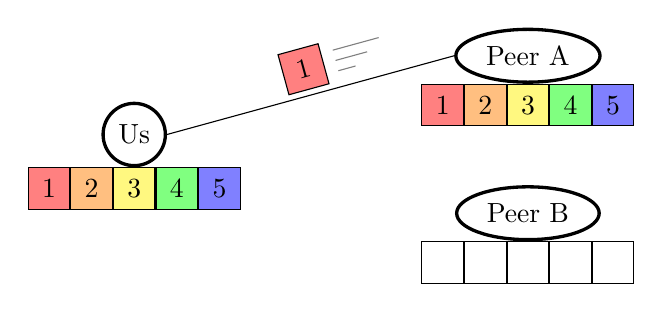
\begin{tikzpicture}
        \node[ellipse,very thick,draw=black] (peera) at (5,1) {Peer A};
        \node[rectangle,draw=black,fill=yellow!50,anchor=north,minimum size=1.5em] (peera-piece3) at ($(peera.south)$) {3};
        \node[rectangle,draw=black,fill=orange!50,anchor=east,minimum size=1.5em] (peera-piece2) at ($(peera-piece3.west)$) {2};
        \node[rectangle,draw=black,fill=red!50,anchor=east,minimum size=1.5em] (peera-piece1) at ($(peera-piece2.west)$) {1};
        \node[rectangle,draw=black,fill=green!50,anchor=west,minimum size=1.5em] (peera-piece4) at ($(peera-piece3.east)$) {4};
        \node[rectangle,draw=black,fill=blue!50,anchor=west,minimum size=1.5em] (peera-piece5) at ($(peera-piece4.east)$) {5};

        \node[ellipse,very thick,draw=black] (peerb) at (5,-1) {Peer B};
        \node[rectangle,draw=black,anchor=north,minimum size=1.5em] (peerb-piece3) at ($(peerb.south)$) {\phantom{3}};
        \node[rectangle,draw=black,anchor=east,minimum size=1.5em] (peerb-piece2) at ($(peerb-piece3.west)$) {\phantom{2}};
        \node[rectangle,draw=black,anchor=east,minimum size=1.5em] (peerb-piece1) at ($(peerb-piece2.west)$) {\phantom{1}};
        \node[rectangle,draw=black,anchor=west,minimum size=1.5em] (peerb-piece4) at ($(peerb-piece3.east)$) {\phantom{4}};
        \node[rectangle,draw=black,anchor=west,minimum size=1.5em] (peerb-piece5) at ($(peerb-piece4.east)$) {\phantom{5}};

        \node[circle,very thick,draw=black] (us) at (0,0) {Us};
        \node[rectangle,draw=black,fill=yellow!50,anchor=north,minimum size=1.5em] (us-piece3) at ($(us.south)$) {3};
        \node[rectangle,draw=black,fill=orange!50,anchor=east,minimum size=1.5em] (us-piece2) at ($(us-piece3.west)$) {2};
        \node[rectangle,draw=black,fill=red!50,anchor=east,minimum size=1.5em] (us-piece1) at ($(us-piece2.west)$) {1};
        \node[rectangle,draw=black,fill=green!50,anchor=west,minimum size=1.5em] (us-piece4) at ($(us-piece3.east)$) {4};
        \node[rectangle,draw=black,fill=blue!50,anchor=west,minimum size=1.5em] (us-piece5) at ($(us-piece4.east)$) {5};

        \draw ($(us.east)$) -- ($(peera.west)$) node [midway,sloped,above=2pt,rectangle,draw=black,fill=red!50,minimum size=1.5em] (movingpiece) {1};
        \coordinate (peeraoffset) at ($(peera.west) - (us.east)$);
        \coordinate (startoffset) at ($0.04*(peeraoffset)$);
        \draw [gray] ($(movingpiece.north east)!.75!(movingpiece.south east) + (startoffset)$) -- ($(movingpiece.north east)!.75!(movingpiece.south east) + 0.1*(peeraoffset)$);
        \draw [gray] ($(movingpiece.east) + (startoffset)$) -- ($(movingpiece.east) + 0.15*(peeraoffset)$);
        \draw [gray] ($(movingpiece.north east)!.25!(movingpiece.south east) + (startoffset)$) -- ($(movingpiece.north east)!.25!(movingpiece.south east) + 0.2*(peeraoffset)$);
    \end{tikzpicture}
\end{document}
